% ================================= RESULTADOS ================================
\section{Resultados}\label{sec:resultados}

\subsection{Caracterização do conjunto analisado}
A análise principal usa os 312 pacientes rotulados: 197 vivos aos cinco anos e 115 óbitos (36,9\%). Todos os modelos foram avaliados nesses 312 pacientes, com imputação ou tratamento nativo dos ausentes. A Tabela~\ref{tab:caracterizacao} compara os dois grupos. Os pacientes que morreram eram mais velhos e tinham, na linha de base, bilirrubina muito mais alta, albumina mais baixa, tempo de protrombina mais longo, edema e ascite mais frequentes e estágio histológico mais avançado, o mesmo padrão que deu origem às variáveis do Escore de Mayo.

\begin{table}[htbp]
\centering
\caption{Características da linha de base por desfecho em cinco anos (312 pacientes rotulados).}
\label{tab:caracterizacao}
\small
\renewcommand{\arraystretch}{1.12}
\begin{adjustbox}{max width=\linewidth}
\begin{tabular}{@{}lccc@{}}
\toprule
\textbf{Variável} & \textbf{Vivos (n = 197)} & \textbf{Óbitos (n = 115)} & \textbf{Ausentes} \\
\midrule
Idade (anos) & 49,8 (42,6--56,0) & 53,9 (46,7--61,8) & 0 \\
Sexo masculino (\%) & 8,1 & 15,7 & 0 \\
Bilirrubina (mg/dL) & 0,90 (0,60--1,60) & 4,40 (2,30--10,15) & 0 \\
Albumina (g/dL) & 3,67 (3,48--3,94) & 3,26 (3,01--3,52) & 0 \\
Tempo de protrombina (s) & 10,45 (10,00--11,00) & 11,10 (10,53--11,97) & 2 \\
Edema presente (\%) & 7,6 & 34,8 & 0 \\
Ascite (\%)\textsuperscript{a} & 1,9 & 23,5 & 68 \\
Plaquetas ($10^3$/mm$^3$) & 266,5 (202,5--336,3) & 214 (156--292) & 11 \\
Estágio histológico & 3 (2--3) & 4 (3--4) & 6 \\
\bottomrule
\end{tabular}
\end{adjustbox}
\par\vspace{3pt}{\footnotesize\color{cinzasec}Fonte: elaboração própria. Valores numéricos em mediana (intervalo interquartil). \textsuperscript{a}Entre os pacientes com o dado; ausente nos 68 rotulados fora do ensaio.}
\end{table}

\subsection{Comparação do desempenho dos modelos}
A Tabela~\ref{tab:resultados} apresenta o desempenho na validação cruzada 5 x 5. A referência principal, a regressão logística com as 5 variáveis de Mayo, teve AUROC média de 0,906 e estimativas de calibração próximas das ideais (CITL de $-$0,01 e inclinação de 1,04). A maior AUROC nominal foi a da regressão penalizada com 17 variáveis (0,915). \textit{Random forest} e XGBoost ficaram entre 0,891 e 0,903 nas configurações principais. A dispersão entre partições (desvio de 0,035 a 0,051) é maior do que qualquer diferença entre modelos.

\begin{table}[htbp]
\centering
\caption{Desempenho na validação cruzada 5 x 5 (média $\pm$ desvio entre as 25 partições; 312 pacientes).}
\label{tab:resultados}
\footnotesize
\renewcommand{\arraystretch}{1.16}
\setlength{\tabcolsep}{4pt}
\begin{adjustbox}{max width=\linewidth}
\begin{tabular}{@{}lccccc@{}}
\toprule
\textbf{Modelo} & \textbf{AUROC} & \textbf{AP} & \textbf{Brier} & \textbf{CITL} & \textbf{Inclinação} \\
\midrule
\textit{Mayo 1989, prob. original}\textsuperscript{a} & 0,910 $\pm$ 0,040 & 0,879 $\pm$ 0,054 & 0,121 $\pm$ 0,023 & 0,33 $\pm$ 0,18 & 1,56 $\pm$ 0,44 \\
\textit{Mayo 1989, recalibrado}\textsuperscript{a} & 0,910 $\pm$ 0,040 & 0,879 $\pm$ 0,054 & 0,112 $\pm$ 0,028 & 0,00 $\pm$ 0,31 & 1,10 $\pm$ 0,33 \\
\textbf{RL, 5 var. (referência)} & \textbf{0,906 $\pm$ 0,044} & \textbf{0,871 $\pm$ 0,061} & \textbf{0,115 $\pm$ 0,032} & \textbf{$-$0,01 $\pm$ 0,33} & \textbf{1,04 $\pm$ 0,36} \\
RL \textit{elastic net}, 17 var. & 0,915 $\pm$ 0,035 & 0,880 $\pm$ 0,051 & 0,121 $\pm$ 0,024 & 0,00 $\pm$ 0,25 & 1,74 $\pm$ 0,91 \\
RF, 5 var. & 0,893 $\pm$ 0,047 & 0,852 $\pm$ 0,066 & 0,130 $\pm$ 0,030 & 0,01 $\pm$ 0,27 & 1,27 $\pm$ 0,60 \\
RF, 17 var. & 0,903 $\pm$ 0,044 & 0,862 $\pm$ 0,069 & 0,124 $\pm$ 0,026 & 0,02 $\pm$ 0,21 & 1,57 $\pm$ 0,58 \\
XGBoost, 5 var. & 0,891 $\pm$ 0,051 & 0,852 $\pm$ 0,072 & 0,126 $\pm$ 0,033 & 0,04 $\pm$ 0,26 & 1,09 $\pm$ 0,34 \\
XGBoost, 17 var. & 0,895 $\pm$ 0,042 & 0,854 $\pm$ 0,064 & 0,126 $\pm$ 0,028 & 0,04 $\pm$ 0,26 & 1,15 $\pm$ 0,41 \\
RF, 17 var., pré-proc. da RL\textsuperscript{b} & 0,907 $\pm$ 0,042 & 0,868 $\pm$ 0,063 & 0,122 $\pm$ 0,024 & 0,00 $\pm$ 0,20 & 1,52 $\pm$ 0,60 \\
XGBoost, 17 var., pré-proc. da RL\textsuperscript{b} & 0,899 $\pm$ 0,039 & 0,855 $\pm$ 0,053 & 0,126 $\pm$ 0,027 & 0,07 $\pm$ 0,33 & 1,04 $\pm$ 0,46 \\
\bottomrule
\end{tabular}
\end{adjustbox}
\par\vspace{3pt}{\footnotesize\color{cinzasec}Fonte: elaboração própria. \textsuperscript{a}Referência histórica: coeficientes estimados com os mesmos pacientes, inclusive os de teste. \textsuperscript{b}Análise de sensibilidade com o pré-processamento da regressão logística (RL).}
\end{table}

A Tabela~\ref{tab:incremental} mostra o valor incremental sobre a referência. Em nenhuma das cinco comparações o IC de Bonferroni excluiu zero. A regressão penalizada com 17 variáveis teve a maior diferença nominal (+0,009) e superou a referência em 60\% das partições. Os modelos de AM ficaram nominalmente abaixo da referência ($-$0,013 a 0,000) e a superaram em apenas 20\% a 40\% das partições. O XGBoost com 5 variáveis teve IC 95\% inteiramente negativo, mas o IC de Bonferroni incluiu zero.

\begin{table}[htbp]
\centering
\caption{Valor incremental em AUROC sobre a regressão logística com as 5 variáveis de Mayo.}
\label{tab:incremental}
\footnotesize
\renewcommand{\arraystretch}{1.16}
\setlength{\tabcolsep}{4pt}
\begin{adjustbox}{max width=\linewidth}
\begin{tabular}{@{}lccccc@{}}
\toprule
\textbf{Modelo} & \textbf{$\Delta$AUROC} & \textbf{IC 95\%} & \textbf{IC 99\% (Bonferroni)} & \textbf{$\Delta$ por partição} & \textbf{Partições com ganho} \\
\midrule
RL \textit{elastic net}, 17 var. & +0,009 & [$-$0,010; 0,030] & [$-$0,017; 0,035] & +0,009 $\pm$ 0,027 & 60\% \\
RF, 5 var. & $-$0,013 & [$-$0,029; 0,003] & [$-$0,035; 0,009] & $-$0,013 $\pm$ 0,019 & 24\% \\
RF, 17 var. & 0,000 & [$-$0,018; 0,016] & [$-$0,022; 0,024] & $-$0,003 $\pm$ 0,018 & 40\% \\
XGBoost, 5 var. & $-$0,013 & [$-$0,027; $-$0,001] & [$-$0,031; 0,003] & $-$0,016 $\pm$ 0,019 & 20\% \\
XGBoost, 17 var. & $-$0,006 & [$-$0,025; 0,012] & [$-$0,030; 0,017] & $-$0,011 $\pm$ 0,019 & 24\% \\
\bottomrule
\end{tabular}
\end{adjustbox}
\par\vspace{3pt}{\footnotesize\color{cinzasec}Fonte: elaboração própria. Intervalos por \textit{bootstrap} pareado de pacientes (2.000 reamostragens), condicionais às predições fora da partição e, por isso, exploratórios. Leitura em todas as linhas: sem evidência de diferença.}
\end{table}

No desenho 2 x 2, as 12 variáveis extras acrescentaram cerca de 0,01 de AUROC nominal em cada família (regressão: 0,906 para 0,915; \textit{random forest}: 0,893 para 0,903; XGBoost: 0,891 para 0,895), sem contraste inferencial próprio. Na leitura vertical, a regressão teve a maior AUROC nominal nas duas colunas. Com o pré-processamento da regressão, \textit{random forest} e XGBoost com 17 variáveis também não mostraram ganho sobre a regressão penalizada ($-$0,006, IC de Bonferroni de 97,5\% [$-$0,023; 0,011]; e $-$0,013 [$-$0,030; 0,004]). Nominalmente, esse pré-processamento elevou a AUROC das árvores (de 0,903 para 0,907 e de 0,895 para 0,899), mas esse efeito não foi testado diretamente.

A Figura~\ref{fig:roc} mostra a distribuição das AUROCs por partição, as curvas ROC sobre as predições fora da partição e a calibração por decis de risco. As curvas ROC praticamente se sobrepõem. Na calibração, a probabilidade original do Escore de Mayo fica acima da diagonal em quase toda a faixa, ou seja, subestima o risco observado, enquanto os demais modelos ficam próximos da diagonal, com oscilações entre decis; com cerca de 31 pacientes por decil, a figura é descritiva e não traz bandas de incerteza.

\begin{figure}[htbp]
\centering
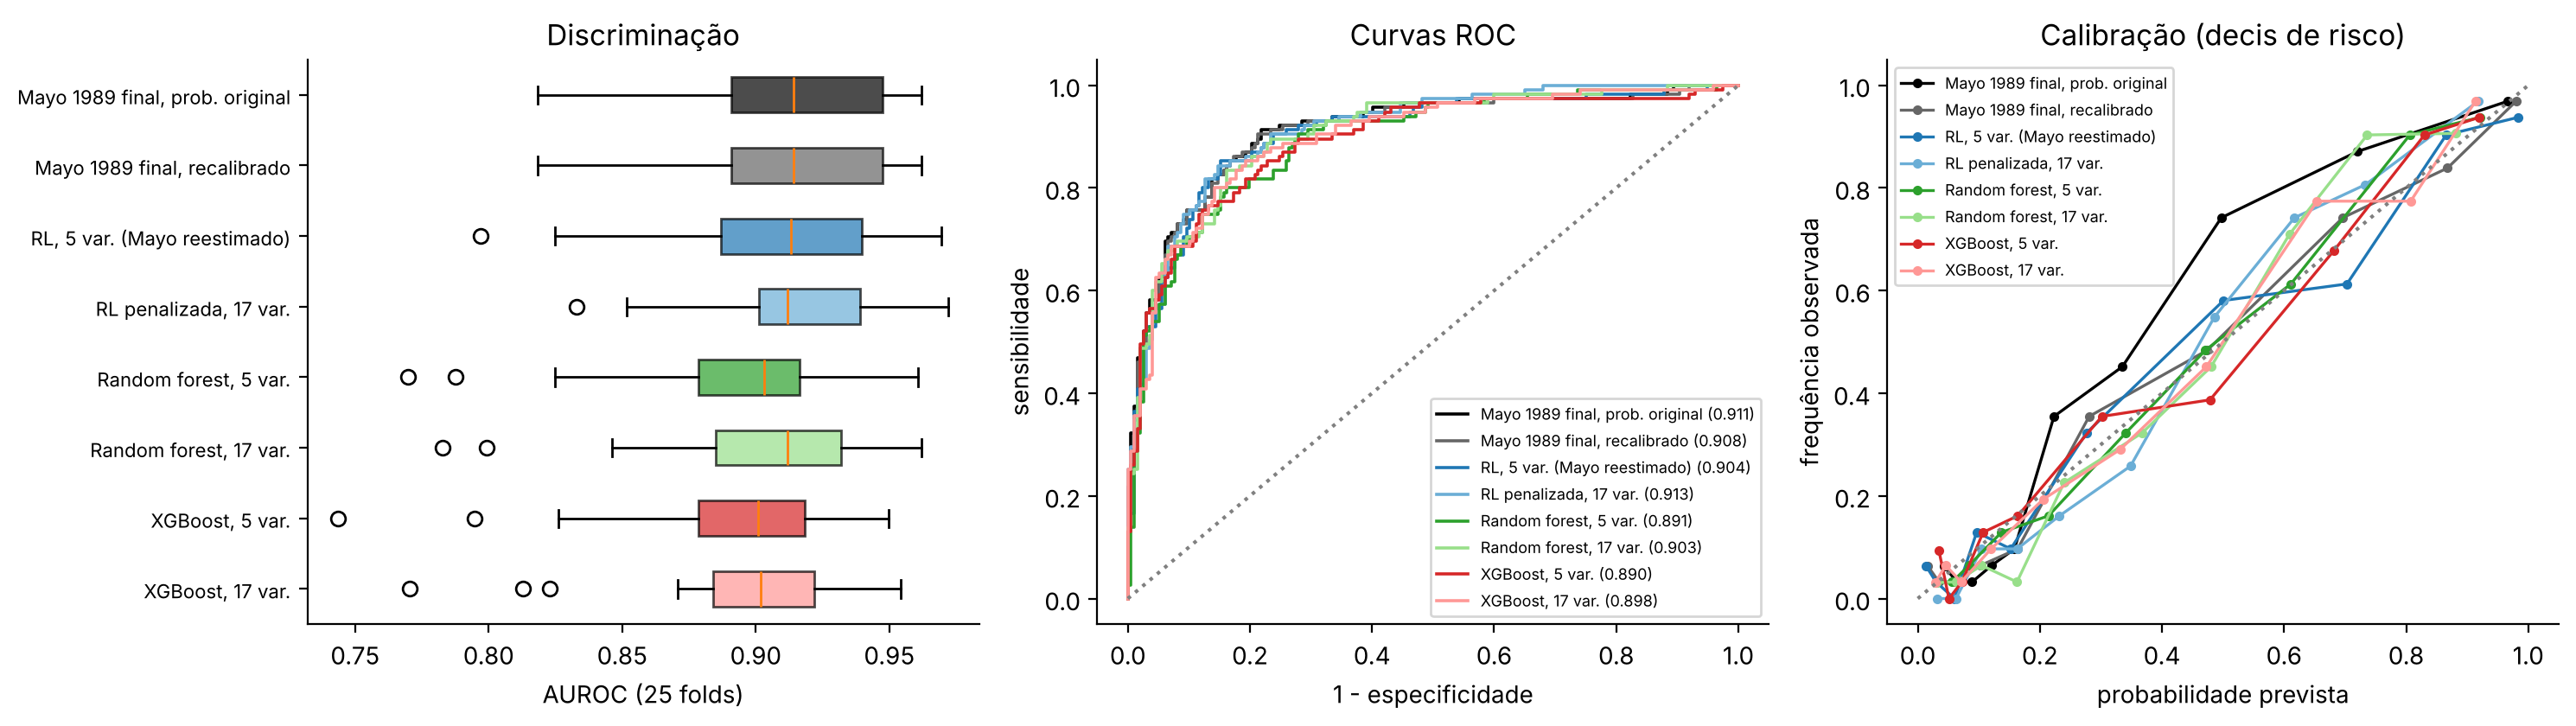
\includegraphics[width=\linewidth]{figuras/discriminacao_roc_calibracao.png}
\caption{AUROC nas 25 partições (esquerda), curvas ROC sobre as predições fora da partição (centro) e calibração por decis de risco (direita).}
\label{fig:roc}
\par\vspace{3pt}{\footnotesize\color{cinzasec}Fonte: elaboração própria; 312 pacientes. A AUROC da legenda é calculada sobre as predições médias e difere ligeiramente da média por partição da Tabela~\ref{tab:resultados}.}
\end{figure}

\subsection{Análise de erros e resultados complementares}
\textbf{Erros no limiar de 0,5.} A Tabela~\ref{tab:limiar} traduz as probabilidades em decisões, usando o limiar de 0,5 sobre as predições fora da partição. O limiar é ilustrativo, pois nenhum limiar clínico foi definido para esta população. A referência identificou 89 dos 115 óbitos (sensibilidade de 0,774), com 23 falsos positivos entre 197 sobreviventes. Os modelos de AM das configurações principais deixaram de identificar de 32 a 34 óbitos, contra 26 da referência. A probabilidade original do Escore de Mayo teve a maior precisão (0,873), mas a menor sensibilidade (0,600), consequência direta da subestimação do risco: com probabilidades baixas demais, menos pacientes ultrapassam o limiar.

\begin{table}[htbp]
\centering
\caption{Medidas de classificação no limiar de 0,5 (predições fora da partição; 115 óbitos e 197 sobreviventes).}
\label{tab:limiar}
\small
\renewcommand{\arraystretch}{1.14}
\begin{adjustbox}{max width=\linewidth}
\begin{tabular}{@{}lccccc@{}}
\toprule
\textbf{Modelo} & \textbf{Precisão} & \textbf{Sensibilidade} & \textbf{Especificidade} & \textbf{F1} & \textbf{Óbitos não detectados} \\
\midrule
\textit{Mayo 1989, prob. original} & 0,873 & 0,600 & 0,949 & 0,711 & 46 \\
\textit{Mayo 1989, recalibrado} & 0,821 & 0,757 & 0,904 & 0,787 & 28 \\
\textbf{RL, 5 var.} & \textbf{0,795} & \textbf{0,774} & \textbf{0,883} & \textbf{0,784} & \textbf{26} \\
RL \textit{elastic net}, 17 var. & 0,819 & 0,748 & 0,904 & 0,782 & 29 \\
RF, 5 var. & 0,794 & 0,704 & 0,893 & 0,747 & 34 \\
RF, 17 var. & 0,781 & 0,713 & 0,883 & 0,745 & 33 \\
XGBoost, 5 var. & 0,786 & 0,704 & 0,888 & 0,743 & 34 \\
XGBoost, 17 var. & 0,790 & 0,722 & 0,888 & 0,755 & 32 \\
\bottomrule
\end{tabular}
\end{adjustbox}
\par\vspace{3pt}{\footnotesize\color{cinzasec}Fonte: elaboração própria. Sensibilidade equivale à revocação (\textit{recall}). Análise descritiva, sem intervalos de confiança.}
\end{table}

\textbf{Referência histórica.} Contra a probabilidade original do Escore de Mayo publicado, a regressão reestimada com 5 variáveis ficou em $-$0,007 (IC de Bonferroni [$-$0,018; 0,003]), e \textit{random forest} e XGBoost com 5 variáveis ficaram abaixo ($-$0,021 cada, com IC de Bonferroni que exclui zero). Essa comparação favorece o escore, cujos coeficientes foram estimados com os pacientes de teste, e por isso não sustenta inferências sobre o valor do escore em pacientes novos.

\textbf{Validação quase externa.} A Tabela~\ref{tab:quase} apresenta o desempenho no teste com os 68 pacientes não randomizados. O comparador histórico válido é o modelo inicial de Dickson, estimado sem esses pacientes (AUROC de 0,865). A mortalidade no teste (44,1\%) foi maior que no treino (34,8\%), e quase todos os modelos subestimaram o risco (CITL entre +0,30 e +0,85). A exceção foi o XGBoost com 17 variáveis, que perdeu discriminação (0,845) e superestimou o risco (CITL de $-$0,81). Com o pré-processamento da regressão, o mesmo algoritmo chegou a 0,888. Com 68 pacientes e 30 óbitos, nenhum intervalo de confiança foi calculado, e diferenças de alguns centésimos não devem ser interpretadas. A análise é descritiva e serve para sinalizar quedas grandes de discriminação e desvios de calibração.

\begin{table}[htbp]
\centering
\caption{Validação quase externa: treino nos 244 pacientes do ensaio, teste nos 68 não randomizados (30 óbitos).}
\label{tab:quase}
\small
\renewcommand{\arraystretch}{1.14}
\begin{adjustbox}{max width=\linewidth}
\begin{tabular}{@{}lccccc@{}}
\toprule
\textbf{Modelo} & \textbf{AUROC} & \textbf{AP} & \textbf{Brier} & \textbf{CITL} & \textbf{Inclinação} \\
\midrule
Mayo 1989 inicial (n = 312), recalibrado & 0,865 & 0,847 & 0,155 & 0,33 & 0,83 \\
RL, 5 var. & 0,878 & 0,844 & 0,144 & 0,30 & 0,88 \\
RL \textit{elastic net}, 17 var. & 0,874 & 0,859 & 0,172 & 0,46 & 2,27 \\
RF, 5 var. & 0,882 & 0,876 & 0,145 & 0,41 & 1,15 \\
RF, 17 var. & 0,896 & 0,876 & 0,145 & 0,30 & 1,49 \\
XGBoost, 5 var. & 0,879 & 0,870 & 0,145 & 0,38 & 0,99 \\
XGBoost, 17 var. & 0,845 & 0,842 & 0,179 & $-$0,81 & 1,00 \\
RF, 17 var., pré-proc. da RL & 0,897 & 0,882 & 0,149 & 0,79 & 0,98 \\
XGBoost, 17 var., pré-proc. da RL & 0,888 & 0,878 & 0,150 & 0,85 & 0,66 \\
\bottomrule
\end{tabular}
\end{adjustbox}
\par\vspace{3pt}{\footnotesize\color{cinzasec}Fonte: elaboração própria. Os coeficientes finais de Mayo foram estimados com os 418 pacientes, inclusive os 68 do teste, e foram omitidos desta tabela (estão no repositório).}
\end{table}

\textbf{Vazamento por \texttt{N\_Days}.} No enquadramento da competição do Kaggle (três classes, 418 pacientes, XGBoost com 17 variáveis), incluir \texttt{N\_Days} como entrada reduziu o \textit{log loss} de 0,753 $\pm$ 0,089 para 0,645 $\pm$ 0,086, elevou a AUROC macro de 0,788 $\pm$ 0,043 para 0,822 $\pm$ 0,045 e a acurácia de 0,721 $\pm$ 0,037 para 0,763 $\pm$ 0,032 (Figura~\ref{fig:vazamento}). O ganho vem de uma informação que não existe no momento da predição.

\begin{figure}[htbp]
\centering
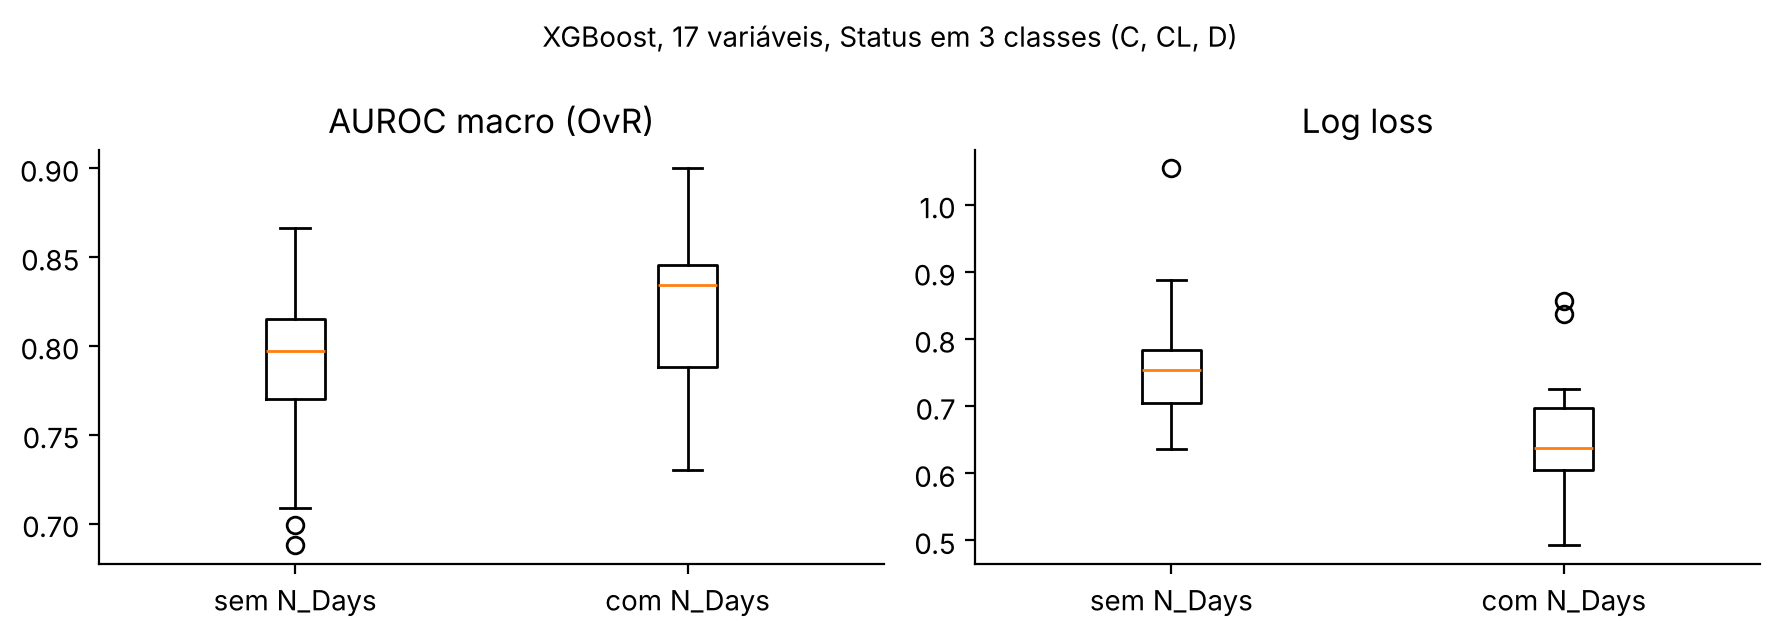
\includegraphics[width=0.78\linewidth]{figuras/vazamento_n_days.png}
\caption{Efeito de usar \texttt{N\_Days} como entrada no enquadramento de três classes (25 partições).}
\label{fig:vazamento}
\par\vspace{3pt}{\footnotesize\color{cinzasec}Fonte: elaboração própria; 418 pacientes.}
\end{figure}
